%
% GNU courseware, XIN YUAN, 2017
%

\documentclass[11pt]{beamer}
%graphics
\usepackage{graphicx}
\usepackage{animate}
%table
\usepackage{colortbl}
%beamer
\usepackage{beamerthemesplit}
%xeCJK
\usepackage[BoldFont,SlantFont,CJKchecksingle]{xeCJK}
\setCJKmainfont[BoldFont=SimHei,SlantedFont=KaiTi]{SimSun}
\setCJKsansfont[BoldFont=SimHei,SlantedFont=KaiTi]{SimSun}
\setCJKmonofont[ItalicFont={Adobe Fangsong Std}]{SimSun}
\setCJKfamilyfont{zhsong}{SimSun}
%\setCJKfamilyfont{zhhei}{Adobe Song Std}
\setCJKfamilyfont{zhhei}{SimHei}
%\setCJKfamilyfont{zhhei}{Adobe Heiti Std}
\setCJKfamilyfont{zhkai}{KaiTi}
\setCJKfamilyfont{zhfs}{FangSong}
%theme
\usetheme{berkeley}

\parindent 1.5em

%title
\title{C++项目管理及工程实践}
\author{袁昕}
\date{\today}

\begin{document}

\frame{\titlepage}

%tables

\section*{大纲}

\frame{
\centerline{\textbf{\Huge{\textcolor[rgb]{0.0, 0.0, 1.0}{C++的问题和团队协作开发}}}}
}

\frame{\tableofcontents}

%sections

%
% GNU courseware, XIN YUAN, 2018
%

\section{C++编程的思考}

\frame{
\centerline{\textbf{\Huge{C++编程的思考}}}
}

\frame{\frametitle{C++发展简史}
{\CJKfamily{zhkai}
\begin{enumerate}
\item<1-> 第一阶段是从80年代到1995年,是传统意义上的面向对象语言,流行在工业领域。
\item<2-> 第二阶段是从1995年到2000年,泛型程序设计在C++中占据了越来越大的比重。同时,
Java、C\#等语言出现,以及硬件价格的大规模下降,C++的份额受到了一定的冲击。
\item<3-> 第三阶段是从2000年至今,各种现代语言特性的不断加入,使得C++出现了发展历史上
又一个新的高峰。C++的份额呈现出稳定的态势。
\end{enumerate}
}
}

\frame{\frametitle{C++标准}
{\CJKfamily{zhkai}
\begin{itemize}
\item<1-> C++原先没有国际标准。1998年,C++标准委员会成立,并通过国际标准组织
(International Standard Organization, ISO)颁布了C++程序设计语言的国际标准
ISO/IEC 1988-1998,通常称作ANSI/ISO C++。委员会随后每5年视实际需要更新一次标准。
\item<2-> 2003年,C++标准进行了一次更新,被称为ISO/IEC 14882,通称为C++03。
2011年,C++0x最终也成为了新的国际标准,被称为C++11,国际标准化组织发布的名称是
ISO/IEC 14882:2011, Information technonly--Programming languages--C++ Edition:3。
\item<3-> 随着现代语言特性的不断加入,新的标准不断出现:C++14,C++17。
\end{itemize}
}
}

\frame{\frametitle{C++对C语言的增强}
{\CJKfamily{zhkai}
\begin{itemize}
\item<1-> 类型检查更为严格。
\item<2-> 增加了面向对象的机制。
\item<3-> 增加了泛型编程的机制。
\item<4-> 增加了异常处理。
\item<5-> 增加了运算符重载。
\item<6-> 增加了标准模板库。
\end{itemize}
}
}

\frame{\frametitle{C++的编程范式}
{\CJKfamily{zhkai}
\begin{itemize}
\item<1-> C子语言。
\item<2-> 面向对象的C++语言。
\item<3-> 泛型编程语言。
\item<4-> 函数式语言。
\end{itemize}
}
}

\frame{\frametitle{C++语言的优点}
{\CJKfamily{zhkai}
\begin{itemize}
\item<1-> 编写C++程序无需复杂的程序设计环境,可以完全命令行方式进行。
\item<2-> C++没有对运行平台的限定,可编写移植性好的程序。
\item<3-> C++和C语言完全兼容,C程序员可以方便地从C平滑过渡到C++语言。
\item<4-> C++是静态类型的语言,不使用会带来额外开销的特性,相对众多其他面向对象的语言,
具有相当高的性能。
\item<5-> C++适合用来设计多种用途的程序。
\item<6-> C++支持多种程序设计风格。
\end{itemize}
}
}

\frame{\frametitle{C++语言的缺点}
{\CJKfamily{zhkai}
\begin{itemize}
\item<1-> C++是一门复杂的语言,这门语言拥有过多的特性从而难以彻底掌握。
\item<2-> C++提供的某些库难以学习、掌握并应用于实际编程中。
\item<3-> C++语言不是上下文无关的文法。
\item<4-> 源代码、静态库、动态库、可执行文件可能互不兼容。
\item<5-> C++依然受制于文件包含的编译模型,这是计算机发展早期内存较小时代的无奈选择。
\item<6-> C++并不是纯粹的面向对象语言,在进行程序设计时,它并没有从系统的对象角度去考虑,
而是从静态的类型建模出发的。
\end{itemize}
}
}

\frame{\frametitle{C++语言的缺点}
{\CJKfamily{zhkai}
\begin{itemize}
\item<1-> 容易失控的模板编程。
\item<2-> STL写出来的代码难以理解、不美观。
\item<3-> C++语言支持多种编程范式。
\item<4-> C++支持的多种程序设计风格导致源代码在不同的程序员之间交流变得非常困难,可维护性差。
\item<5-> C++原先不支持多线程原语。
\item<6-> C++程序的复杂性导致大中型C++程序的正确性难于保证。
\end{itemize}
}
}

\frame{\frametitle{C++的库}
{\CJKfamily{zhkai}
C++的很多特性都是以库 (如C运行时库CRT,标准模板库STL) 或其他的形式提供的,
而没有直接添加到语言本身里面。
}
}

\frame{\frametitle{C++的学习过程}
{\CJKfamily{zhkai}
\begin{enumerate}
\item<1-> 基本的语法、关键字、运算符、表达式等的熟练应用。
\item<2-> 面向对象的基本概念及熟练应用。
\item<3-> 设计模式及模板的熟练应用,包括模板库STL的应用。
\item<4-> 模板元编程 (即生成式模板编程及函数式编程) 的熟练应用。
\item<5-> 熟练掌握C++预处理期图灵完备的宏的应用。
\item<6-> 熟练地混合运用各种范式。
\end{enumerate}
}
}

\frame{\frametitle{C++的应用场景}
{\CJKfamily{zhkai}
C++语言目前出现了精英化发展的趋势,即它退出了那些可用可不用领域的程序开发,
如面向消费类的大型应用程序。剩下那些附加值高和难度高的领域,包括底层的系统级程序开发,
如操作系统、数据库后端、网站后端,以及实时性要求高的程序,
如工业控制、卫星控制、导弹控制等专业领域。另外,C++也还活跃在学术界的科研活动中。
}
}

\frame{\frametitle{C++应用场合}
{\CJKfamily{zhkai}
\begin{itemize}
\item<1-> 服务器端服务程序的开发
\item<2-> 组件服务程序的开发
\item<3-> 控制台程序的开发
\item<4-> 组件化桌面程序的开发,可无缝迁移到云端
\item<5-> 专业软件的开发
\end{itemize}
}
}

\frame{\frametitle{C++实战原则}
{\CJKfamily{zhkai}
\begin{enumerate}
\item<1-> 对C++语言的编程进行规范化的改造。对于不同类型的应用程序,采用不同的范式来开发。
\item<2-> 对于底层系统级的程序,如操作系统或者是实时性要求高的应用程序,
采取偏向C语言面向过程的范式来开发。可引入简单的类概念及函数指针绑定到类的技术。
\item<3-> 对于大中型的高层应用程序,在面向对象范式、泛型范式、函数范式中,
选取一个合适的自定义的子集,加以改进和规范化,同时保证开发效率和执行效率。
\end{enumerate}
}
}

\frame{\frametitle{C++编程改进}
{\CJKfamily{zhkai}
\begin{enumerate}
\item<1-> 编程风格和规范
\item<2-> 基本数据类型和复合类型
\item<3-> 类对象的内存设计
\item<4-> 类的组成
\item<5-> 异常
\item<6-> 共享库
\item<7-> 字符串和国际化
\end{enumerate}
}
}

\frame{\frametitle{编程风格和规范}
{\CJKfamily{zhkai}
\begin{itemize}
\item<1-> 对头文件和实现文件的程序定义。
\item<2-> 将全局变量、类的静态成员变量、含有静态局部变量的函数或方法定义在cpp文件中。
\item<3-> 使用预编译头技术。
\item<4-> 结合使用驼峰命名、匈牙利命名和Linux风格的命名。命名体现自解释。
\item<5-> 必要的文档化注释。
\end{itemize}
}
}

\frame{\frametitle{数据类型}
{\CJKfamily{zhkai}
\begin{itemize}
\item<1-> 定义跨平台,占用字节数明确的基本数据类型。
\item<2-> 定义指针相关的整数类型。
\item<3-> 取消共用体。
\item<4-> 全局变量和全局函数可以用类的静态成员、静态方法来取代。
\item<5-> 统一使用类的概念。
\item<6-> 引入接口。
\item<7-> 枚举转化为真正的类型。
\item<8-> 类或结构的对齐。
\end{itemize}
}
}

\frame{\frametitle{类对象的语义}
{\CJKfamily{zhkai}
\begin{itemize}
\item<1-> 类对象的生命周期。
\item<2-> 值语义和引用语义。
\item<3-> 考虑右值引用。
\item<4-> 浅拷贝和深拷贝。
\item<5-> 类方法的参数使用引用语义,类方法的返回值使用值语义。
\end{itemize}
}
}

\frame{\frametitle{类对象的内存设计}
{\CJKfamily{zhkai}
\begin{itemize}
\item<1-> 化动态内存管理为静态内存管理。
\item<2-> 使用智能指针。
\item<3-> 注意循环引用问题。
\item<4-> 使用迭代器访问容器类对象的每个元素。
\end{itemize}
}
}

\frame{\frametitle{类的组成}
{\CJKfamily{zhkai}
\begin{itemize}
\item<1-> 通过属性访问数据成员,不直接公开成员对象。
\item<2-> 提供方法。
\item<3-> 支持触发事件,即观察者模式。
\item<4-> 不重载操作符。
\item<5-> 支持多继承,接口继承,静多态。
\end{itemize}
}
}

\frame{\frametitle{异常}
{\CJKfamily{zhkai}
\begin{itemize}
\item<1-> 从一个自定义的基类派生,尽量不使用虚方法,各个方法体内不要抛出异常。
\item<2-> 对于潜在的逻辑错误(如指针指向NULL对象),程序员有责任修复错误,
因此不在程序中检查,让其抛出。
\item<3-> 对于运行时错误,则根据需要在合适的地方捕获异常,或者不处理。
服务程序要捕获所有异常。常见运行时错误包括内存不足和加法乘法的溢出。
\item<4-> 工程设置中不启用浮点数异常。在程序中处理无效的浮点数。
\item<5-> 析构方法不抛出异常。
\item<6-> 构造方法可以抛出异常,但要注意内存泄漏问题。
\item<7-> 在确定不抛异常的函数/方法定义的末尾添加异常过滤器说明throw()。
\end{itemize}
}
}

\frame{\frametitle{共享库}
{\CJKfamily{zhkai}
\begin{itemize}
\item<1-> 引入版本号。
\item<2-> 使用扩展关键字引出函数,不加序号。
\item<3-> 导出函数或方法的所有参数和返回值要注意字节对齐。
\item<4-> 进行组件化的设计,导出组件类,使用接口访问组件。
\item<5-> 支持远程组件,组件所在共享库可运行在本机或者其他计算机的其他进程中。
\end{itemize}
}
}

\frame{\frametitle{字符串和国际化}
{\CJKfamily{zhkai}
\begin{itemize}
\item<1-> 使用固定长度的数组和动态数组来实现字符串。
\item<2-> 需要国际化的数据单独设计为数据文件,在程序中使用特殊标记。
\item<3-> 需要国际化的数据设计为带版本号的共享库,在程序中使用特殊标记。
\end{itemize}
}
}

%end


%
% GNU courseware, XIN YUAN, 2018
%

\section{团队协作}

\frame{
\centerline{\textbf{\Huge{团队协作}}}
}

\frame{\frametitle{角色分工}
\begin{table}[htbp]
\centering
\begin{tabular}{|p{0.3\textwidth}<{\centering}|p{0.6\textwidth}|}
\hline
\textbf{角色} & \textbf{分工}\\
\hline
\rowcolor[rgb]{0.0, 0.8, 0.8}
项目经理 & 产品设计和工程监督\\
\hline
架构师 & 软件架构设计\\
\hline
\rowcolor[rgb]{0.0, 0.8, 0.8}
程序员 & 程序开发\\
\hline
测试员 & 软件测试\\
\hline
\end{tabular}
\end{table}
}

\frame{\frametitle{工具链}
\begin{table}[htbp]
\centering
\begin{tabular}{|p{0.3\textwidth}<{\centering}|p{0.6\textwidth}|}
\hline
\textbf{名称} & \textbf{工具}\\
\hline
\rowcolor[rgb]{0.0, 0.8, 0.8}
版本控制 & Git, fossil\\
\hline
持续集成 & Jenkins, Appveyor\\
\hline
\rowcolor[rgb]{0.0, 0.8, 0.8}
构建工具 & CMake, QMake\\
\hline
规范检查 & cpplint\\
\hline
\rowcolor[rgb]{0.0, 0.8, 0.8}
静态分析 & cppcheck\\
\hline
复杂度分析 & cppncss\\
\hline
\rowcolor[rgb]{0.0, 0.8, 0.8}
单元测试覆盖率 & OpenCppCoverage, gcov\\
\hline
\end{tabular}
\end{table}
}

\frame{\frametitle{工作流程}
单人工作和多人协作是不同的。

~

\begin{itemize}
\item<1-> 瀑布流程:需求-分析-概要设计-详细设计-编码实现-测试-发布-反馈
\item<2-> 敏捷流程:用户故事-场景-测试用例-迭代-反馈
\end{itemize}
}

\frame{\frametitle{工作流程}
\begin{minipage}[t]{\textwidth}
git flow:
\end{minipage}

~

\uncover<2->{
\noindent
\begin{minipage}[b]{\textwidth}
\begin{figure}[hb]
\centering
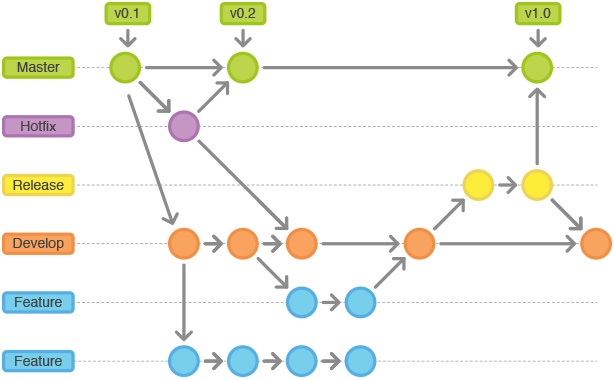
\includegraphics[width=0.8\textwidth]{topics/team-files/wf-git.png}
\end{figure}
\end{minipage}
}
}

\frame{\frametitle{工作流程}
\begin{minipage}[t]{\textwidth}
github flow:
\end{minipage}

~

\uncover<2->{
\noindent
\begin{minipage}[b]{\textwidth}
\begin{figure}[hb]
\centering
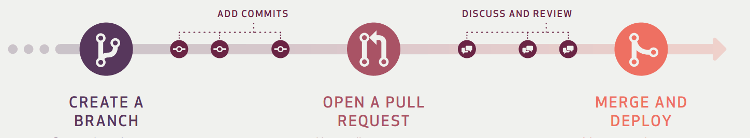
\includegraphics[width=0.8\textwidth]{topics/team-files/wf-github.png}
\end{figure}
\end{minipage}
}
}

\frame{\frametitle{GitHub工作流程}
\begin{figure}[hb]
\centering
\animategraphics[height=1.5in, autoplay, controls]{1}{topics/team-files/wf-github-a}{1}{6}
\end{figure}
}

\frame{\frametitle{工作流程}
\begin{minipage}[t]{\textwidth}
GitLab工作流程分为持续发布和版本发布:
\end{minipage}

~

\begin{minipage}[b]{\textwidth}
\noindent
\begin{figure}[hb]
\centering
\uncover<2->{
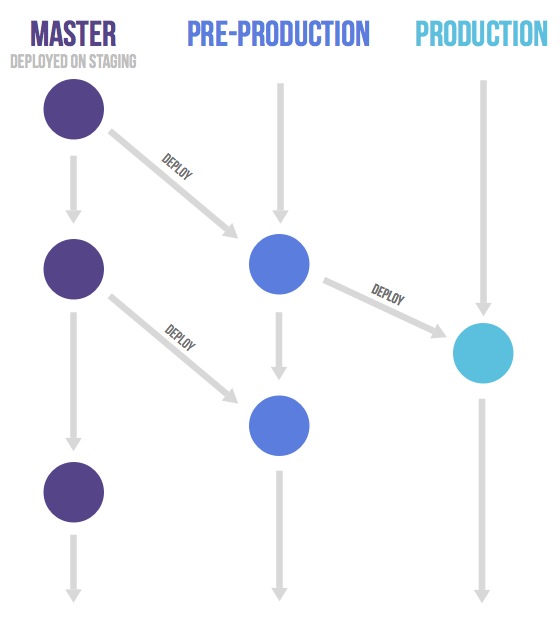
\includegraphics[width=0.4\textwidth]{topics/team-files/wf-gitlab1.png}
}
~
\uncover<3->{
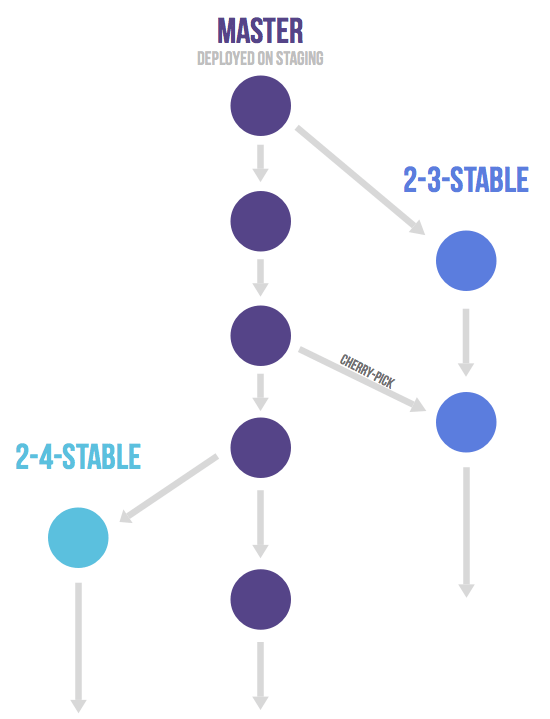
\includegraphics[width=0.4\textwidth]{topics/team-files/wf-gitlab2.png}
}
\end{figure}
\end{minipage}
}

\frame{\frametitle{工作流程}
\begin{minipage}[t]{\textwidth}
fossil flow:
\end{minipage}

~

\uncover<2->{
\noindent
\begin{minipage}[b]{\textwidth}
\begin{figure}[hb]
\centering
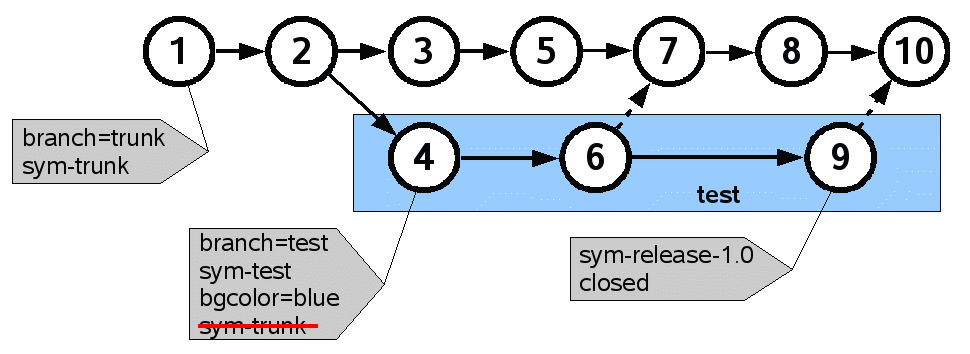
\includegraphics[width=0.8\textwidth]{topics/team-files/wf-fossil.png}
\end{figure}
\end{minipage}
}
}

\frame{\frametitle{工作流程}

一般地,某一个人做一个或多个功能或者修订一个或多个issue/ticket就要开一个新的分支,
完成后关闭或删除。
}

\frame{\frametitle{文档}
\begin{table}[htbp]
\centering
\begin{tabular}{|p{0.6\textwidth}|p{0.3\textwidth}|}
\hline
\textbf{内容} & \textbf{格式}\\
\hline
\rowcolor[rgb]{0.0, 0.9, 0.8}
需求分析 & Markdown(可以在线协作)\\
\hline
技术分析 & Markdown(可以在线协作)\\
\hline
\rowcolor[rgb]{0.0, 0.9, 0.8}
规划分析(思维导图,规划系统和行动全景图) & Markdown\\
\hline
测试计划 & Markdown(可以在线协作)\\
\hline
\rowcolor[rgb]{0.0, 0.9, 0.8}
甘特图/燃尽图 & LaTex\\
\hline
用例图 & LaTex \\
\hline
\rowcolor[rgb]{0.0, 0.9, 0.8}
类图 & LaTex\\
\hline
顺序协作图 & LaTex\\
\hline
\end{tabular}
\end{table}
}

%end


%end

\frame{\frametitle{结束}
\centerline{\textbf{\Huge{结束!}}}
}

\frame{\frametitle{版权申明}

本作品采用知识共享 署名-非商业性使用-禁止演绎 3.0 中国大陆 许可协议进行许可。
要查看该许可协议,可访问 http://creativecommons.org/licenses/by-nc-nd/3.0/cn/ 或者
写信到 Creative Commons, PO Box 1866, Mountain View, CA 94042, USA。
}

\end{document}
